\section{Main results}

\begin{table*}[t!]
\centering
\renewcommand{\arraystretch}{1.2}
\renewcommand{\tabcolsep}{1.2mm}
\resizebox{\linewidth}{!}{
  \begin{tabular}{@{}L{2.5cm}|L{1.2cm}|r*{19}{x}|x@{}}
method & train set & aero      & bike      & bird      & boat      & bottle     & bus        & car        & cat        & chair      & cow        & table      & dog        & horse      & mbike      & persn     & plant      & sheep      & sofa       & train      & tv         & mAP       \\
\hline
SPPnet BB \cite{he2014spp}$^\dagger$ &
07 $\setminus$ diff &
73.9 &
72.3 &
62.5 &
51.5 &
44.4 &
74.4 &
73.0 &
74.4 &
42.3 &
73.6 &
57.7 &
70.3 &
74.6 &
74.3 &
54.2 &
34.0 &
56.4 &
56.4 &
67.9 &
73.5 &
63.1 \\
R-CNN BB \cite{rcnn-pami} &
07 &
73.4 &
77.0 &
63.4 &
45.4 &
\bf{44.6} &
75.1 &
78.1 &
79.8 &
40.5 &
73.7 &
62.2 &
79.4 &
78.1 &
73.1 &
64.2 &
\bf{35.6} &
66.8 &
67.2 &
70.4 &
\bf{71.1} &
66.0 \\
\hline
FRCN [ours] &
07 &
74.5 &
78.3 &
69.2 &
53.2 &
36.6 &
77.3 &
78.2 &
82.0 &
40.7 &
72.7 &
67.9 &
79.6 &
79.2 &
73.0 &
69.0 &
30.1 &
65.4 &
70.2 &
75.8 &
65.8 &
66.9 \\
FRCN [ours] &
07 $\setminus$ diff &
74.6 &
\bf{79.0} &
68.6 &
57.0 &
39.3 &
79.5 &
\bf{78.6} &
81.9 &
\bf{48.0} &
74.0 &
67.4 &
80.5 &
80.7 &
74.1 &
69.6 &
31.8 &
67.1 &
68.4 &
75.3 &
65.5 &
68.1 \\
FRCN [ours] &
07+12 &
\bf{77.0} &
78.1 &
\bf{69.3} &
\bf{59.4} &
38.3 &
\bf{81.6} &
\bf{78.6} &
\bf{86.7} &
42.8 &
\bf{78.8} &
\bf{68.9} &
\bf{84.7} &
\bf{82.0} &
\bf{76.6} &
\bf{69.9} &
31.8 &
\bf{70.1} &
\bf{74.8} &
\bf{80.4} &
70.4 &
\bf{70.0} \\
\end{tabular}
}
\vspace{0.05em}
\caption{{\bf VOC 2007 test} detection average precision (\%). All methods use \vggsixteen. Training set key: {\bf 07}: VOC07 trainval, {\bf 07 $\setminus$ diff}: {\bf 07} without ``difficult'' examples, {\bf 07+12}: union of {\bf 07} and VOC12 trainval.
$^\dagger$SPPnet results were prepared by the authors of \cite{he2014spp}.}
\tablelabel{voc2007}
\end{table*}

\begin{table*}[t!]
\centering
\renewcommand{\arraystretch}{1.2}
\renewcommand{\tabcolsep}{1.2mm}
\resizebox{\linewidth}{!}{
\begin{tabular}{@{}L{2.5cm}|L{1.2cm}|r*{19}{x}|x@{}}
method & train set & aero      & bike      & bird      & boat      & bottle     & bus        & car        & cat        & chair      & cow        & table      & dog        & horse      & mbike      & persn     & plant      & sheep      & sofa       & train      & tv         & mAP       \\
\hline
BabyLearning &
Prop. &
77.7 &
73.8 &
62.3 &
48.8 &
45.4 &
67.3 &
67.0 &
80.3 &
41.3 &
70.8 &
49.7 &
79.5 &
74.7 &
78.6 &
64.5 &
36.0 &
69.9 &
55.7 &
70.4 &
61.7 &
63.8 \\
R-CNN BB \cite{rcnn-pami} &
12 &
79.3 &
72.4 &
63.1 &
44.0 &
44.4 &
64.6 &
66.3 &
84.9 &
38.8 &
67.3 &
48.4 &
82.3 &
75.0 &
76.7 &
65.7 &
35.8 &
66.2 &
54.8 &
69.1 &
58.8 &
62.9 \\
SegDeepM &
12+seg &
\bf{82.3} &
75.2 &
67.1 &
50.7 &
\bf{49.8} &
71.1 &
69.6 &
88.2 &
42.5 &
71.2 &
50.0 &
85.7 &
76.6 &
81.8 &
69.3 &
\bf{41.5} &
\bf{71.9} &
62.2 &
73.2 &
\bf{64.6} &
67.2 \\
\hline
FRCN [ours] &
12 &
80.1 &
74.4 &
67.7 &
49.4 &
41.4 &
74.2 &
68.8 &
87.8 &
41.9 &
70.1 &
50.2 &
86.1 &
77.3 &
81.1 &
70.4 &
33.3 &
67.0 &
63.3 &
77.2 &
60.0 &
66.1 \\
FRCN [ours] &
07++12 &
82.0 &
\bf{77.8} &
\bf{71.6} &
\bf{55.3} &
42.4 &
\bf{77.3} &
\bf{71.7} &
\bf{89.3} &
\bf{44.5} &
\bf{72.1} &
\bf{53.7} &
\bf{87.7} &
\bf{80.0} &
\bf{82.5} &
\bf{72.7} &
36.6 &
68.7 &
\bf{65.4} &
\bf{81.1} &
62.7 &
\bf{68.8} \\
\end{tabular}
}
\vspace{0.05em}
\caption{{\bf VOC 2010 test} detection average precision (\%).
BabyLearning uses a network based on \cite{Lin2014NiN}.
All other methods use \vggsixteen. Training set key: {\bf 12}: VOC12 trainval, {\bf Prop.}: proprietary dataset, {\bf 12+seg}: {\bf 12} with segmentation annotations, {\bf 07++12}: union of VOC07 trainval, VOC07 test, and VOC12 trainval.
%Results:
%$^\dagger$\url{http://host.robots.ox.ac.uk:8080/anonymous/UKA8XB.html},
%$^\dagger$\url{http://goo.gl/f1vtls},
%$^\ddagger$\url{http://host.robots.ox.ac.uk:8080/anonymous/DGTVGW.html}
%$^\ddagger$\url{http://goo.gl/kyZcnW}
}
\tablelabel{voc2010}
\end{table*}

\begin{table*}[t!]
\centering
\renewcommand{\arraystretch}{1.2}
\renewcommand{\tabcolsep}{1.2mm}
\resizebox{\linewidth}{!}{
  \begin{tabular}{@{}L{2.5cm}|L{1.2cm}|r*{19}{x}|x@{}}
method & train set & aero      & bike      & bird      & boat      & bottle     & bus        & car        & cat        & chair      & cow        & table      & dog        & horse      & mbike      & persn     & plant      & sheep      & sofa       & train      & tv         & mAP       \\
\hline
BabyLearning &
Prop. &
78.0 &
74.2 &
61.3 &
45.7 &
42.7 &
68.2 &
66.8 &
80.2 &
40.6 &
70.0 &
49.8 &
79.0 &
74.5 &
77.9 &
64.0 &
35.3 &
67.9 &
55.7 &
68.7 &
62.6 &
63.2 \\
NUS\_NIN\_c2000 &
Unk. &
80.2 &
73.8 &
61.9 &
43.7 &
\bf{43.0} &
70.3 &
67.6 &
80.7 &
41.9 &
69.7 &
51.7 &
78.2 &
75.2 &
76.9 &
65.1 &
\bf{38.6} &
\bf{68.3} &
58.0 &
68.7 &
63.3 &
63.8 \\
R-CNN BB \cite{rcnn-pami} &
12 &
79.6 &
72.7 &
61.9 &
41.2 &
41.9 &
65.9 &
66.4 &
84.6 &
38.5 &
67.2 &
46.7 &
82.0 &
74.8 &
76.0 &
65.2 &
35.6 &
65.4 &
54.2 &
67.4 &
60.3 &
62.4 \\
\hline
FRCN [ours] &
12 &
80.3 &
74.7 &
66.9 &
46.9 &
37.7 &
73.9 &
68.6 &
87.7 &
41.7 &
71.1 &
51.1 &
86.0 &
77.8 &
79.8 &
69.8 &
32.1 &
65.5 &
63.8 &
76.4 &
61.7 &
65.7 \\
FRCN [ours] &
07++12 &
\bf{82.3} &
\bf{78.4} &
\bf{70.8} &
\bf{52.3} &
38.7 &
\bf{77.8} &
\bf{71.6} &
\bf{89.3} &
\bf{44.2} &
\bf{73.0} &
\bf{55.0} &
\bf{87.5} &
\bf{80.5} &
\bf{80.8} &
\bf{72.0} &
35.1 &
\bf{68.3} &
\bf{65.7} &
\bf{80.4} &
\bf{64.2} &
\bf{68.4} \\
\end{tabular}
}
\vspace{0.05em}
\caption{{\bf VOC 2012 test} detection average precision (\%).
BabyLearning and NUS\_NIN\_c2000 use networks based on \cite{Lin2014NiN}.
All other methods use \vggsixteen. Training set key: see \tableref{voc2010}, {\bf Unk.}: unknown.
%Results:
%$^\dagger$\url{http://host.robots.ox.ac.uk:8080/anonymous/QMSIIY.html},
%$^\ddagger$\url{http://host.robots.ox.ac.uk:8080/anonymous/DCSBZY.html}
%$^\dagger$\url{http://goo.gl/weNq2Z},
%$^\ddagger$\url{http://goo.gl/o1tZ10}
}
\tablelabel{voc2012}
\end{table*}



Three main results support this paper's contributions:
\begin{enumerate}
  \itemsep0em
  \item State-of-the-art mAP on VOC07, 2010, and 2012
  \item Fast training and testing compared to R-CNN, SPPnet
  \item Fine-tuning conv layers in \vggsixteen improves mAP
\end{enumerate}

\subsection{Experimental setup}
\seclabel{setup}
Our experiments use three pre-trained ImageNet models that are available online.\footnote{\url{https://github.com/BVLC/caffe/wiki/Model-Zoo}}
The first is the CaffeNet (essentially AlexNet \cite{krizhevsky2012imagenet}) from R-CNN \cite{girshick2014rcnn}.
We alternatively refer to this CaffeNet as model \Sm, for ``small.''
The second network is VGG\_CNN\_M\_1024 from \cite{Chatfield14}, which has the same depth as \Sm, but is wider.
We call this network model \Med, for ``medium.''
The final network is the very deep \vggsixteen model from \cite{simonyan2015verydeep}.
Since this model is the largest, we call it model \Lg.
In this section, all experiments use \emph{single-scale} training and testing ($s = 600$; see \secref{scale} for details).

\subsection{VOC 2010 and 2012 results}
On these datasets, we compare Fast R-CNN (\emph{FRCN}, for short) against the top methods on the \texttt{comp4} (outside data) track from the public leaderboard (\tableref{voc2010}, \tableref{voc2012}).\footnote{\url{http://host.robots.ox.ac.uk:8080/leaderboard} (accessed April 18, 2015)}
For the NUS\_NIN\_c2000 and BabyLearning methods, there are no associated publications at this time and we could not find exact information on the ConvNet architectures used; they are variants of the Network-in-Network design \cite{Lin2014NiN}.
All other methods are initialized from the same pre-trained \vggsixteen network.
%We show results when training on the VOC12 trainval image set as well as an augmented dataset that includes all annotated images in VOC07.

Fast R-CNN achieves the top result on VOC12 with a mAP of 65.7\% (and 68.4\% with extra data).
It is also two orders of magnitude faster than the other methods, which are all based on the ``slow'' R-CNN pipeline.
On VOC10, SegDeepM \cite{Zhu2015segDeepM} achieves a higher mAP than Fast R-CNN (67.2\% vs. 66.1\%).
SegDeepM is trained on VOC12 trainval plus segmentation annotations; it is designed to boost R-CNN accuracy by using a Markov random field to reason over R-CNN detections and segmentations from the O$_2$P \cite{o2p} semantic-segmentation method.
Fast R-CNN can be swapped into SegDeepM in place of R-CNN, which may lead to better results.
When using the enlarged 07++12 training set (see \tableref{voc2010} caption), Fast R-CNN's mAP increases to 68.8\%, surpassing SegDeepM.

\subsection{VOC 2007 results}
On VOC07, we compare Fast R-CNN to R-CNN and SPPnet.
All methods start from the same pre-trained \vggsixteen network and use bounding-box regression.
The \vggsixteen SPPnet results were computed by the authors of \cite{he2014spp}.
SPPnet uses five scales during both training and testing.
The improvement of Fast R-CNN over SPPnet illustrates that even though Fast R-CNN uses single-scale training and testing, fine-tuning the conv layers provides a large improvement in mAP (from 63.1\% to 66.9\%).
%Moreover, single-scale testing significantly speeds up detection.
R-CNN achieves a mAP of 66.0\%.
%Fast R-CNN surpasses R-CNN, at 66.9\%.
%These results are pragmatically valuable given how much faster and easier Fast R-CNN is to train and test, which we discuss next.
As a minor point, SPPnet was trained \emph{without} examples marked as ``difficult'' in PASCAL.
Removing these examples improves Fast R-CNN mAP to 68.1\%.
All other experiments use ``difficult'' examples.

\subsection{Training and testing time}
% Show how long R-CNN and SPP-net take to train and test on VOC07.
Fast training and testing times are our second main result.
\tableref{timing} compares training time (hours), testing rate (seconds per image), and mAP on VOC07 between Fast R-CNN, R-CNN, and SPPnet.
For \vggsixteen, Fast R-CNN processes images 146\X faster than R-CNN without truncated SVD and 213\X faster with it.
Training time is reduced by 9\X, from 84 hours to 9.5.
Compared to SPPnet, Fast R-CNN trains \vggsixteen 2.7\X faster (in 9.5 vs. 25.5 hours) and tests 7\X faster without truncated SVD or 10\X faster with it.
Fast R-CNN also eliminates hundreds of gigabytes of disk storage, because it does not cache features.

\begin{table}[h!]
\begin{center}
\setlength{\tabcolsep}{3pt}
\renewcommand{\arraystretch}{1.2}
\resizebox{\linewidth}{!}{
\small
\begin{tabular}{l|rrr|rrr|r}
  & \multicolumn{3}{c|}{Fast R-CNN} & \multicolumn{3}{c|}{R-CNN} & \multicolumn{1}{c}{SPPnet} \\
  & \Sm & \Med & \Lg & \Sm & \Med & \Lg & $^\dagger$\Lg \\
%  & \multicolumn{3}{c|}{\Sm} & \multicolumn{3}{c|}{\Med} & \multicolumn{3}{c}{\Lg}  \\
\hline
train time (h) & \bf{1.2} & 2.0 & 9.5 &
22 & 28 & 84 & 25 \\
train speedup & \bf{18.3\X} & 14.0\X & 8.8\X &
1\X & 1\X & 1\X & 3.4\X \\
\hline
test rate (s/im) & 0.10 & 0.15 & 0.32 &
9.8 & 12.1 & 47.0 & 2.3 \\
~$\rhd$ with SVD & \bf{0.06} & 0.08 & 0.22 &
- & - & - & - \\
\hline
test speedup & 98\X & 80\X & 146\X &
1\X & 1\X & 1\X & 20\X \\
~$\rhd$ with SVD & 169\X & 150\X & \bf{213\X} &
- & - & - & - \\
\hline
VOC07 mAP & 57.1 & 59.2 & \bf{66.9} &
58.5 & 60.2 & 66.0 & 63.1 \\
~$\rhd$ with SVD & 56.5 & 58.7 & 66.6 &
- & - & - & - \\
\end{tabular}
}
\end{center}
\caption{Runtime comparison between the same models in Fast R-CNN, R-CNN, and SPPnet.
Fast R-CNN uses single-scale mode.
SPPnet uses the five scales specified in \cite{he2014spp}.
$^\dagger$Timing provided by the authors of \cite{he2014spp}.
Times were measured on an Nvidia K40 GPU.
}
\tablelabel{timing}
\vspace{-1em}
\end{table}
% R-CNN VGG16 training time: 18 hrs (fine-tuning) + 63 hrs (feature extraction) + 3 hrs (SVM and bbox reg) = 84 hrs
% R-CNN CNN_M training time: 10.5 hrs (fine-tuning) + 14.3 hrs (feature extraction) + 3 hrs (SVM and bbox reg) = 28 hrs
% R-CNN CaffeNet training time: 8 hrs (fine-tuning) + 11.1 hrs (feature extraction) + 3 hours (SVM and bbox reg) = 22 hrs

% Runtime results from Kaiming:
%1. Yes, it is 5 scales as those scales in the original SPP paper. We do not have single-scale result, but we can run the experiment if you feel it is useful.
%2. The conv feature extraction is 2s for 5 scales without flipping (as for test) and 4s for 5 scales with flipping (as for training). The fine-tuning depends on the quality of hard disk, because the fc training time is small and reading features from disks can be overhead. In our local machine with good hard disks, the fine-tuning time is about 16 hours. SVM takes 2 hours, and bbox takes 2hours.
%3. Inference is about 2.3s, for 2s on conv features of all 5 scales, and 0.3 s for spp/fc layers.

% Training time: (feature extraction) 4s/image * 5011 images = 5.6 hours
% + (fine-tuning) 16 hours + (SVM) 2 hours + (bbox reg) 2 hours \approx 25.5 hours

% Test time: 2.3s / image



%\begin{table}[h!]
%\begin{center}
%\setlength{\tabcolsep}{5pt}
%\renewcommand{\arraystretch}{1.1}
%\resizebox{\linewidth}{!}{
%\small
%\begin{tabular}{l|rr|rr|rr}
%  & \multicolumn{2}{c|}{Fast R-CNN} & \multicolumn{2}{c|}{R-CNN} & \multicolumn{2}{c}{SPPnet ZF} \\
%  & \Med & \Lg & \Med & \Lg & 1 scale & 5 scal. \\
%%  & \multicolumn{3}{c|}{\Sm} & \multicolumn{3}{c|}{\Med} & \multicolumn{3}{c}{\Lg}  \\
%\hline
%train time (h) & 2.0 & 9.5 & 27 & 84 & $\approx$3.5$^\dagger$ & $\approx$6$^\dagger$ \\
%train speedup & 13.5x & 8.8x & 1x & 1x & - & - \\
%\hline
%test rate (s/im) & 0.15 & 0.32 & 12.1 & 47.0 & 0.14 & 0.38 \\
%~$\rhd$ with SVD & 0.08 & 0.22 & - & - & - & - \\
%test speedup & 80x & 146x & 1x & 1x & - & - \\
%~$\rhd$ with SVD & 150x & 213x & - & - & - & - \\
%\hline
%VOC07 mAP & 59.2 & 66.9 & 60.2 & 66.0 & 58.0 & 59.2  \\
%~$\rhd$ with SVD & 58.7 & 66.6 & - & - & - & - \\
%\end{tabular}
%}
%\end{center}
%\caption{Runtime comparisons between the same models in Fast R-CNN and R-CNN.
%SPPnet results for models \Med and \Lg are not available; SPPnet uses model ZF, which is similar to model \Sm.
%%Test rate is measured in seconds per image.
%Single-scale training and testing is used for Fast R-CNN.
%$^\dagger$Exact times are not available; we estimated values based on the description in \cite{he2014spp}.
%}
%\tablelabel{timing}
%\end{table}
% R-CNN VGG16 training time: 18 hrs (fine-tuning) + 63 hrs (feature extraction) + 3 hrs (SVM and bbox reg) = 84 hrs
% R-CNN CNN_M training time: 10.5 hrs (fine-tuning) + 14.3 hrs (feature extraction) + 3 hrs (SVM and bbox reg) = 28 hrs

\paragraph{Truncated SVD.}
%\tableref{timing} includes results with and without truncated SVD acceleration.
%For image classification, truncated SVD is primarily useful as a model compression technique to reduce storage space.
%But for detection, it also provides a significant speed-up.
Truncated SVD can reduce detection time by more than 30\% with only a small (0.3 percentage point) drop in mAP and without needing to perform additional fine-tuning after model compression.
\figref{timing} illustrates how using the top $1024$ singular values from the $25088 \times 4096$ matrix in {\vggsixteen}'s fc6 layer and the top $256$ singular values from the $4096 \times 4096$ fc7 layer reduces runtime with little loss in mAP.
Further speed-ups are possible with smaller drops in mAP if one fine-tunes again after compression.
%Here we focus on keeping training as simple as possible.

\begin{figure}[h!]
\centering
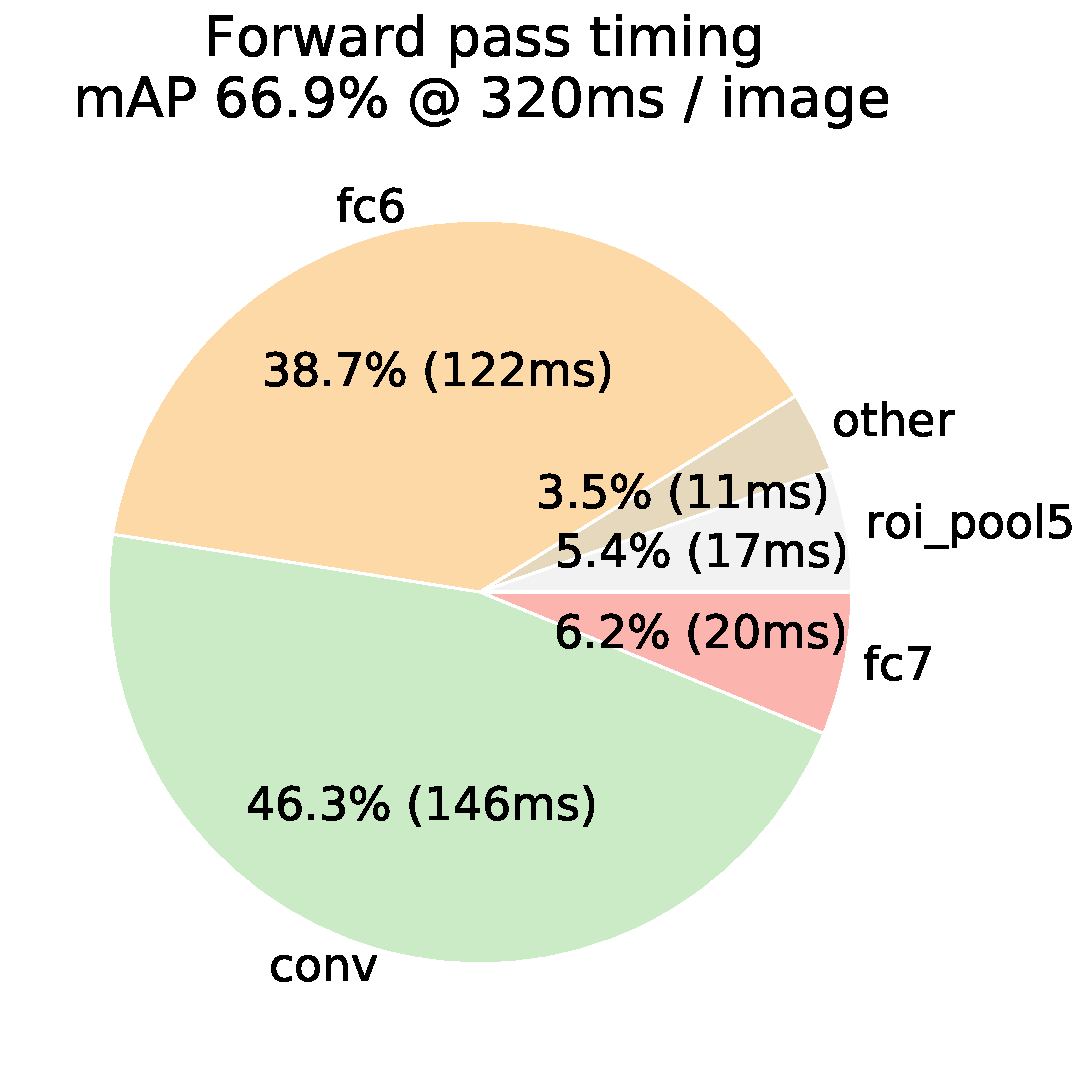
\includegraphics[width=0.49\linewidth,trim=3em 2em 0 0, clip]{figs/layer_timing.pdf}
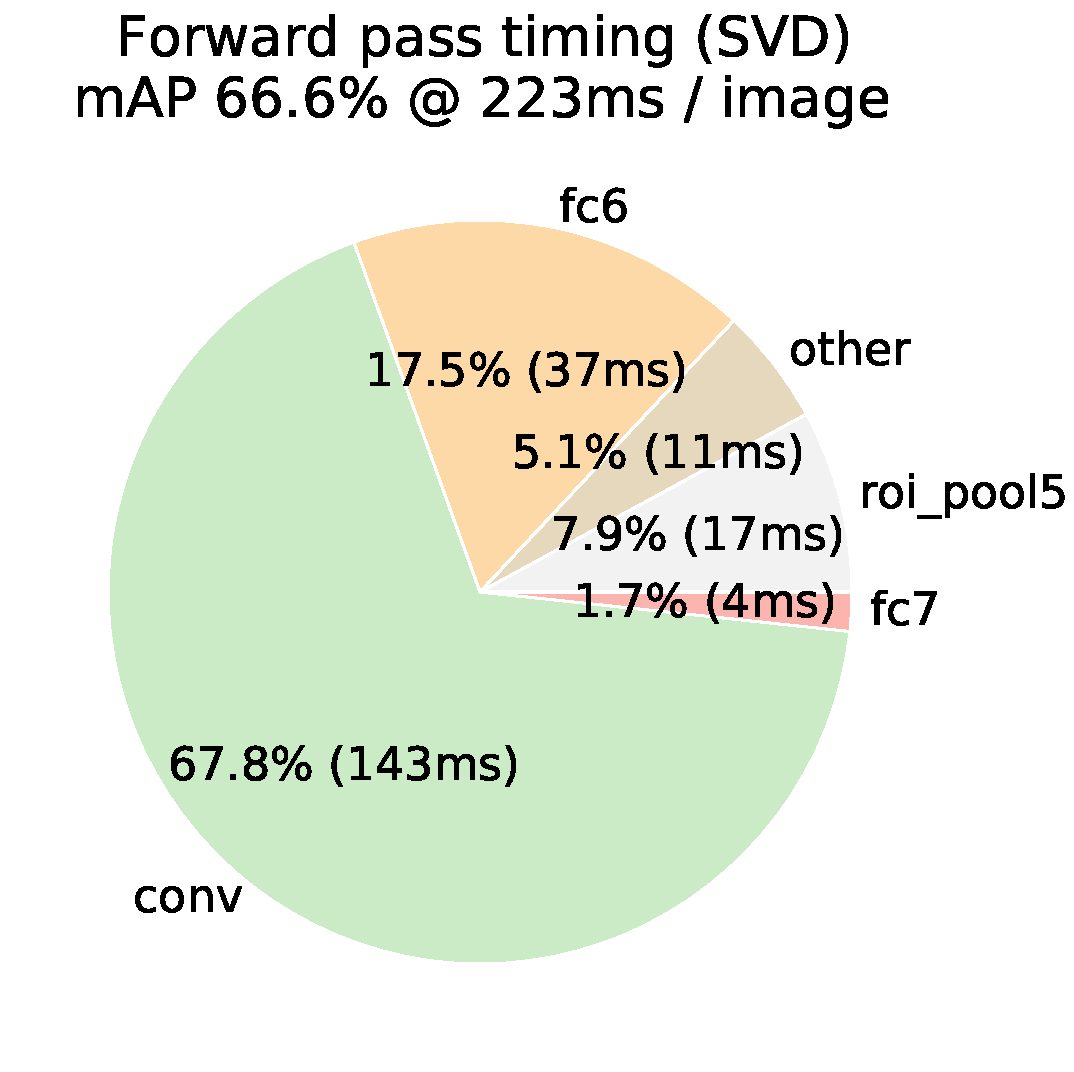
\includegraphics[width=0.49\linewidth,trim=3em 2em 0 0, clip]{figs/layer_timing_svd.pdf}
%\vspace{-1em}
\caption{Timing for \vggsixteen before and after truncated SVD.
Before SVD, fully connected layers fc6 and fc7 take 45\% of the time.}
\figlabel{timing}
\end{figure}

%\begin{table}[h!]
%\begin{center}
%\setlength{\tabcolsep}{6pt}
%\renewcommand{\arraystretch}{1.1}
%\small
%\begin{tabular}{l|rr|rr|rr}
%  & \multicolumn{2}{c|}{\Sm} & \multicolumn{2}{c|}{\Med} & \multicolumn{2}{c}{\Lg} \\
%\hline
%Trunc. SVD? &  & \checkmark &  & \checkmark & & \checkmark \\
%s / image & 0.10 & 0.06 & 0.15 & 0.08 & 0.32 & 0.22 \\
%VOC07 mAP & 57.1 & 56.5 & 59.2 & 58.7 & 66.9 & 66.6
%\end{tabular}
%\end{center}
%\caption{Effects of truncated SVD on test speed and mAP.}
%\tablelabel{svd}
%\end{table}
%
%\tableref{svd} shows results for all three models using the top 1024 and 256 singular values for layers fc6 and fc7, respectively.
%Even though the compression factor increases from \Sm to \Lg, the loss in mAP decreases.

\subsection{Which layers to fine-tune?}
For the less deep networks considered in the SPPnet paper \cite{he2014spp}, fine-tuning only the fully connected layers appeared to be sufficient for good accuracy.
We hypothesized that this result would not hold for very deep networks.
To validate that fine-tuning the conv layers is important for \vggsixteen, we use Fast R-CNN to fine-tune, but \emph{freeze} the thirteen conv layers so that only the fully connected layers learn.
This ablation emulates single-scale SPPnet training and \emph{decreases mAP from 66.9\% to 61.4\%} (\tableref{whichlayers}).
This experiment verifies our hypothesis: training through the \roi pooling layer is important for very deep nets.

\begin{table}[h!]
\begin{center}
\setlength{\tabcolsep}{3pt}
\renewcommand{\arraystretch}{1.1}
\small
\begin{tabular}{l|rrr|r}
  & \multicolumn{3}{c|}{layers that are fine-tuned in model \Lg} & SPPnet \Lg \\
  & $\ge$ fc6 & $\ge$ conv3\_1 & $\ge$ conv2\_1 & $\ge$ fc6 \\
\hline
VOC07 mAP & 61.4 & 66.9 & \bf{67.2} & 63.1 \\
test rate (s/im) & \bf{0.32} & \bf{0.32} & \bf{0.32} & 2.3 \\
\end{tabular}
\end{center}
\caption{Effect of restricting which layers are fine-tuned for \vggsixteen.
Fine-tuning $\ge$ fc6 emulates the SPPnet training algorithm \cite{he2014spp}, but using a single scale.
SPPnet \Lg results were obtained using five scales, at a significant (7\X) speed cost.}
\tablelabel{whichlayers}
\vspace{-0.5em}
\end{table}

Does this mean that \emph{all} conv layers should be fine-tuned? In short, \emph{no}.
In the smaller networks (\Sm and \Med) we find that conv1 is generic and task independent (a well-known fact \cite{krizhevsky2012imagenet}).
Allowing conv1 to learn, or not, has no meaningful effect on mAP.
For \vggsixteen, we found it only necessary to update layers from conv3\_1 and up (9 of the 13 conv layers).
This observation is pragmatic: (1) updating from conv2\_1 slows training by 1.3\X (12.5 vs. 9.5 hours) compared to learning from conv3\_1;
and (2) updating from conv1\_1 over-runs GPU memory.
The difference in mAP when learning from conv2\_1 up was only $+0.3$ points (\tableref{whichlayers}, last column).
All Fast R-CNN results in this paper using \vggsixteen fine-tune layers conv3\_1 and up; all experiments with models \Sm and \Med fine-tune layers conv2 and up.
